\documentclass{article}
\usepackage{graphicx} % Required for inserting images
\usepackage{amsmath}
\usepackage{amssymb}
\usepackage{bm}
\usepackage{xcolor}
\usepackage{listings}
\usepackage[margin=1in]{geometry}
\usepackage{caption}
\usepackage{subcaption}

% --- Python code listing style ---------------------------------------------
\definecolor{codegreen}{rgb}{0.0,0.5,0.0}
\definecolor{codegray}{rgb}{0.5,0.5,0.5}
\definecolor{codepurple}{rgb}{0.58,0.0,0.82}
\definecolor{backcolour}{rgb}{0.96,0.96,0.96}

\lstdefinestyle{python}{
    language=Python,
    backgroundcolor=\color{backcolour},
    commentstyle=\color{codegreen},
    keywordstyle=\color{blue},
    stringstyle=\color{codepurple},
    basicstyle=\ttfamily\footnotesize,
    breakatwhitespace=false,
    breaklines=true,
    captionpos=b,
    keepspaces=true,
    numbers=left,
    numbersep=6pt,
    numberstyle=\tiny\color{codegray},
    showspaces=false,
    showstringspaces=false,
    showtabs=false,
    frame=single,
    tabsize=4,
}
\lstset{style=python}

% --- Notation shortcuts -----------------------------------------------------
\newcommand{\bx}{\mathbf{x}}
\newcommand{\bX}{\mathbf{X}}
\newcommand{\bz}{\mathbf{z}}
\newcommand{\bZ}{\mathbf{Z}}
\newcommand{\bmu}{\bm{\mu}}
\newcommand{\bsigma}{\bm{\sigma}}
\newcommand{\KL}{\mathrm{KL}}

\title{2AMU20 Generative AI \\ Homework 3}
\author{ Triantafyllos Fotoglou :  2153904\\ Ege Ey\"ul K\i rm\i z\i\ : 2254859 \\ Ege Erdal : 2201267\\}
\date{June 2026}

\begin{document}

\maketitle

\section{Introduction}

In this assignment we implement and study a Variational Autoencoder (VAE) for
the MNIST dataset. This section reports our solution to \textbf{Task 1}: a VAE
built from (de)convolutional networks whose conditional data distribution
$p(\bX \mid \bz)$ is a product of independent Gaussians. We describe the
architecture (Task~1a), derive and train the ELBO objective (Task~1b), motivate
our stopping criterion (Task~1c), and show reconstructions of test images
together with samples drawn from the prior (Task~1d).

Our implementation uses \texttt{pytorch} and is organised as a small package:
\texttt{vae/data.py} (MNIST loading and splitting), \texttt{vae/model.py} (the
encoder/decoder networks), \texttt{vae/elbo.py} (the objective),
\texttt{vae/training.py} (the training loop, early stopping and
checkpointing), and \texttt{vae/visualize.py} (the figures). The entry point
\texttt{task1.py} runs the whole pipeline.

\paragraph{Data.} We load MNIST through \texttt{torchvision}. The
\texttt{ToTensor} transform maps the raw \texttt{uint8} pixels in $[0,255]$ to
floats in $[0,1]$, which is exactly the normalisation the task requires. We
verify that the dataset contains $60{,}000$ training and $10{,}000$ testing
images, and split the training set so that the \emph{first} $50{,}000$ images
are used for training and the \emph{last} $10{,}000$ for validation.

\begin{lstlisting}[caption={Loading and splitting MNIST (\texttt{vae/data.py}).}]
transform = transforms.ToTensor()  # maps uint8 [0,255] -> float [0,1]
full_train = MNIST(root=root, train=True, download=download, transform=transform)
test_set = MNIST(root=root, train=False, download=download, transform=transform)

# Verify the dataset sizes the assignment expects.
assert len(full_train) == 60_000 and len(test_set) == 10_000

# First 50.000 -> training, last 10.000 -> validation.
train_set = Subset(full_train, range(0, 50_000))
val_set = Subset(full_train, range(50_000, 60_000))
\end{lstlisting}

\section*{Task 1a --- Model Setup}
\addcontentsline{toc}{section}{Task 1a --- Model Setup}

We use \texttt{pytorch} for both the model and automatic differentiation. The
VAE consists of a convolutional \emph{encoder} that maps an image to the
parameters of the approximate posterior
$q(\bZ \mid \bx) = \mathcal{N}(\bmu_{\text{enc}}(\bx), \mathrm{diag}(\bsigma_{\text{enc}}^2(\bx)))$,
and a transposed-convolutional \emph{decoder} that maps a latent code $\bz$ to
the parameters $\bmu(\bz)$ and $\bsigma^2(\bz)$ of the Gaussian likelihood
$p(\bX \mid \bz)$. We use a latent dimension of $K=16$.

\paragraph{Encoder.} Three stride-2 convolutions reduce the spatial resolution
$28\!\times\!28 \to 14\!\times\!14 \to 7\!\times\!7 \to 4\!\times\!4$ while
increasing the number of channels ($1 \to 32 \to 64 \to 128$). A flattened
linear layer then produces the $K$ posterior means and $K$ posterior
log-variances.

\begin{lstlisting}[caption={Convolutional encoder (\texttt{vae/model.py}).}]
class ConvEncoder(nn.Module):
    def __init__(self, latent_dim: int) -> None:
        super().__init__()
        self.features = nn.Sequential(
            nn.Conv2d(1, 32, kernel_size=4, stride=2, padding=1),    # 28 -> 14
            nn.ReLU(inplace=True),
            nn.Conv2d(32, 64, kernel_size=4, stride=2, padding=1),   # 14 -> 7
            nn.ReLU(inplace=True),
            nn.Conv2d(64, 128, kernel_size=3, stride=2, padding=1),  # 7 -> 4
            nn.ReLU(inplace=True),
        )
        self.flatten = nn.Flatten()
        self.fc_mean = nn.Linear(128 * 4 * 4, latent_dim)
        self.fc_logvar = nn.Linear(128 * 4 * 4, latent_dim)

    def forward(self, x):
        h = self.flatten(self.features(x))
        mean = self.fc_mean(h)
        logvar = self.fc_logvar(h).clamp(-6.0, 2.0)
        return GaussianParams(mean=mean, logvar=logvar)
\end{lstlisting}

\paragraph{Decoder.} A linear layer reshapes $\bz$ into a $128\!\times\!4\!\times\!4$
feature map, which three transposed convolutions upsample back to
$28\!\times\!28$. Two separate $1\!\times\!1$ convolution heads produce the
per-pixel mean $\bmu(\bz)$ and log-variance $\log\bsigma^2(\bz)$. Because the
data lies in $[0,1]$, we pass the mean through a sigmoid; the log-variance is
left unconstrained but clamped to $[-6, 2]$ for numerical stability (the
log-likelihood contains $1/\sigma^2$ and $\log\sigma^2$).

\begin{lstlisting}[caption={Transposed-convolutional decoder (\texttt{vae/model.py}).}]
class ConvDecoder(nn.Module):
    def __init__(self, latent_dim: int) -> None:
        super().__init__()
        self.project = nn.Linear(latent_dim, 128 * 4 * 4)
        self.upsample = nn.Sequential(
            nn.ReLU(inplace=True),
            nn.ConvTranspose2d(128, 64, kernel_size=3, stride=2, padding=1),  # 4 -> 7
            nn.ReLU(inplace=True),
            nn.ConvTranspose2d(64, 32, kernel_size=4, stride=2, padding=1),   # 7 -> 14
            nn.ReLU(inplace=True),
            nn.ConvTranspose2d(32, 32, kernel_size=4, stride=2, padding=1),   # 14 -> 28
            nn.ReLU(inplace=True),
        )
        self.head_mean = nn.Conv2d(32, 1, kernel_size=1)
        self.head_logvar = nn.Conv2d(32, 1, kernel_size=1)

    def forward(self, z):
        h = self.project(z).view(-1, 128, 4, 4)
        h = self.upsample(h)
        mean = torch.sigmoid(self.head_mean(h))           # in [0, 1]
        logvar = self.head_logvar(h).clamp(-6.0, 2.0)
        return GaussianParams(mean=mean, logvar=logvar)
\end{lstlisting}

\paragraph{Optimisation and hyperparameters.} We train by maximising the
(estimated) ELBO with the \textbf{Adam} optimiser. The hyperparameters that
differ from the assignment-neutral defaults are summarised below; all remaining
Adam settings are left at their \texttt{pytorch} defaults
($\beta_1=0.9$, $\beta_2=0.999$).

\begin{center}
\begin{tabular}{ll}
\hline
Hyperparameter & Value \\
\hline
Latent dimension $K$ & $16$ \\
Optimiser & Adam (learning rate $10^{-3}$) \\
Batch size & $128$ \\
Maximum epochs & $100$ \\
Early-stopping patience & $5$ epochs \\
\hline
\end{tabular}
\end{center}

\section*{Task 1b --- Model Training}
\addcontentsline{toc}{section}{Task 1b --- Model Training}

\paragraph{Conditional log-likelihood.} Because $p(\bX \mid \bz)$ is a product
of independent Gaussians, one per feature $d = 1,\dots,D$, the log-likelihood of
a single data-point $\bx$ given a latent code $\bz$ is
\begin{align}
\log p(\bx \mid \bz)
&= \sum_{d=1}^{D} \log \mathcal{N}\!\big(x_d \mid \mu_d(\bz), \sigma_d^2(\bz)\big) \nonumber \\
&= \sum_{d=1}^{D} -\frac{1}{2}\left[
        \log(2\pi) + \log \sigma_d^2(\bz)
        + \frac{\big(x_d - \mu_d(\bz)\big)^2}{\sigma_d^2(\bz)}
   \right],
\end{align}
where $\bmu(\bz)$ and $\bsigma^2(\bz)$ are the outputs of the decoder network
evaluated at $\bz$.

\paragraph{ELBO.} With a standard-normal prior $p(\bZ) = \mathcal{N}(\bm{0}, I)$
and a diagonal-Gaussian posterior, the ELBO of a single data-point is
\begin{equation}
\mathcal{L}(\bx)
= \mathbb{E}_{q(\bZ \mid \bx)}\!\big[\log p(\bx \mid \bz)\big]
  - \KL\!\big(q(\bZ \mid \bx)\,\|\,p(\bZ)\big),
\end{equation}
where the KL term has the closed form
\begin{equation}
\KL\!\big(q(\bZ \mid \bx)\,\|\,p(\bZ)\big)
= \frac{1}{2}\sum_{k=1}^{K}\Big(\sigma_k^2 + \mu_k^2 - 1 - \log \sigma_k^2\Big).
\end{equation}
We approximate the expectation $\mathbb{E}_{q(\bZ \mid \bx)}[\cdot]$ with a
single Monte-Carlo sample $\bz \sim q(\bZ \mid \bx)$ obtained through the
\emph{reparameterisation trick} $\bz = \bmu + \bsigma \odot \bm{\epsilon}$ with
$\bm{\epsilon} \sim \mathcal{N}(\bm{0}, I)$, which makes the sampling step
differentiable.

\begin{lstlisting}[caption={The ELBO terms (\texttt{vae/elbo.py}).}]
def gaussian_log_likelihood(x, px):
    var = torch.exp(px.logvar)
    log_prob = -0.5 * (LOG_2PI + px.logvar + (x - px.mean) ** 2 / var)
    return log_prob.flatten(start_dim=1).sum(dim=1)   # sum over D features

def kl_to_standard_normal(q):
    var = torch.exp(q.logvar)
    kl = 0.5 * (var + q.mean ** 2 - 1.0 - q.logvar)
    return kl.sum(dim=1)                              # sum over K latents

def elbo(x, q, px):
    log_likelihood = gaussian_log_likelihood(x, px)
    kl = kl_to_standard_normal(q)
    return (log_likelihood - kl).mean()               # batch-averaged ELBO
\end{lstlisting}

\paragraph{Training loop.} We maximise the ELBO (i.e.\ minimise its negative)
with Adam. After every epoch we evaluate the ELBO on the full training and
validation splits. Crucially, the evaluation is wrapped in
\texttt{torch.no\_grad()} so that computing the validation ELBO never tracks
gradients and therefore cannot leak into training.

\begin{lstlisting}[caption={Core of the training loop (\texttt{vae/training.py}).}]
optimiser = torch.optim.Adam(model.parameters(), lr=learning_rate)
for epoch in range(1, max_epochs + 1):
    model.train()
    for x, _ in data.train_loader:
        x = x.to(device)
        optimiser.zero_grad()
        q, _, px = model(x)
        loss = -elbo(x, q, px).elbo   # maximise ELBO == minimise its negative
        loss.backward()
        optimiser.step()

    # End-of-epoch ELBO on both splits, without tracking gradients.
    train_eval = evaluate(model, data.train_loader, device)
    val_eval = evaluate(model, data.val_loader, device)
\end{lstlisting}

\begin{lstlisting}[caption={Gradient-free evaluation (\texttt{vae/training.py}).}]
@torch.no_grad()
def evaluate(model, loader, device):
    model.eval()
    total_elbo, total_count = 0.0, 0
    for x, _ in loader:
        x = x.to(device)
        q, _, px = model(x)
        total_elbo += elbo(x, q, px).elbo.item() * x.size(0)
        total_count += x.size(0)
    return total_elbo / total_count
\end{lstlisting}

\paragraph{ELBO curve.} Figure~\ref{fig:elbo} shows how the per-image ELBO on
the $50{,}000$ training images and the $10{,}000$ validation images evolves with
the number of training epochs. Both curves increase steeply during the first
few epochs and then flatten. The training and validation curves track each
other closely (the small, stable gap indicates no significant overfitting),
and the best validation ELBO of $\mathbf{1322.4}$ is reached at epoch~$35$.

\begin{figure}[h]
    \centering
    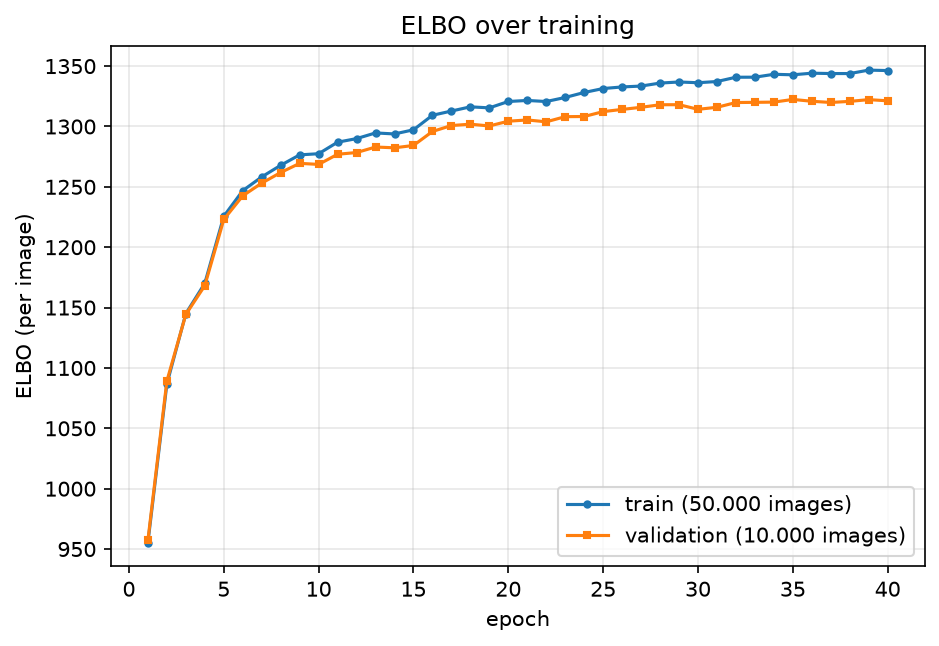
\includegraphics[width=0.75\textwidth]{outputs/task1_elbo.png}
    \caption{ELBO (per image) on the training and validation splits as a
    function of the training epoch. The ELBO increases with training and
    plateaus, with the validation curve closely following the training curve.}
    \label{fig:elbo}
\end{figure}

\section*{Task 1c --- Stopping Criterion}
\addcontentsline{toc}{section}{Task 1c --- Stopping Criterion}

We use \textbf{early stopping on the validation ELBO}: after each epoch we
compare the current validation ELBO to the best one seen so far, and we
terminate training once it has \emph{not improved for $5$ consecutive epochs}
(the \emph{patience}). The parameters that achieved the best validation ELBO
are saved to disk and restored at the end of training.

\paragraph{Motivation.} The validation ELBO measures how well the model
generalises to data it was not trained on. Stopping as soon as this quantity
stops improving (i)~prevents the model from overfitting to the training set,
and (ii)~saves compute by not running unnecessary epochs. Using a patience of
several epochs makes the criterion robust to the small epoch-to-epoch noise
caused by the single-sample Monte-Carlo estimate of the ELBO. In our run,
training stopped at epoch~$40$ (best validation ELBO at epoch~$35$). To avoid
ever having to re-train, the best model is checkpointed with
\texttt{torch.save} and can be reloaded with \texttt{torch.load}.

\begin{lstlisting}[caption={Early stopping and checkpointing (\texttt{vae/training.py}).}]
if val_eval.elbo > best_val_elbo:
    best_val_elbo = val_eval.elbo
    epochs_without_improvement = 0
    save_checkpoint(model, checkpoint_path)         # keep the best model
else:
    epochs_without_improvement += 1
    if epochs_without_improvement >= patience:      # patience = 5
        break                                       # stop training
\end{lstlisting}

\section*{Task 1d --- Model Testing}
\addcontentsline{toc}{section}{Task 1d --- Model Testing}

To reconstruct a testing image $\bx$ we follow the procedure in the
assignment: we (1)~pass $\bx$ through the encoder to obtain $q(\bZ \mid \bx)$,
(2)~draw a sample $\bz \sim q(\bZ \mid \bx)$, (3)~pass $\bz$ through the decoder
to obtain $p(\bX \mid \bz)$, and (4)~sample an image $\bx' \sim p(\bX \mid \bz)$.

\begin{lstlisting}[caption={Reconstruction of a test image (\texttt{vae/visualize.py}).}]
q = model.encode(originals)            # 1. q(Z | x)
z = model.reparameterise(q)            # 2. z ~ q(Z | x)
px = model.decode(z)                   # 3. p(X | z)
reconstructions = sample_image(px)     # 4. x' ~ p(X | z), clamped to [0, 1]
\end{lstlisting}

Figure~\ref{fig:recon} shows the first $32$ testing images alongside their
reconstructions in an $8\!\times\!8$ grid. The originals occupy rows
$1,3,5,7$ and each reconstruction is placed directly below its original in rows
$2,4,6,8$. The reconstructions clearly recover the correct digit identity and
overall shape; the residual graininess is expected because we \emph{sample}
$\bx' \sim p(\bX \mid \bz)$ rather than displaying the mean $\bmu(\bz)$.

\begin{figure}[h]
    \centering
    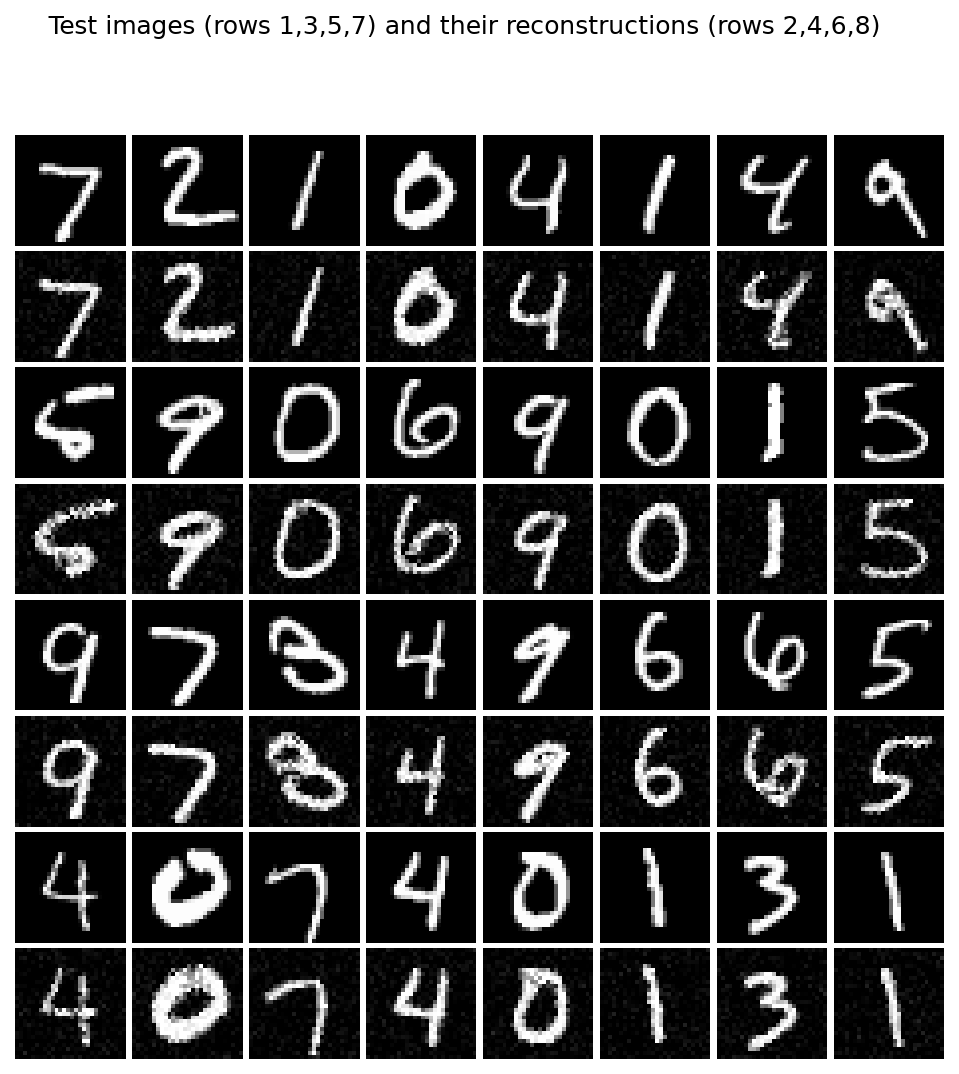
\includegraphics[width=0.7\textwidth]{outputs/task1_reconstructions.png}
    \caption{First $32$ testing images (odd rows) and their reconstructions
    (even rows), arranged in an $8\!\times\!8$ grid.}
    \label{fig:recon}
\end{figure}

We also generate completely new images by sampling $\bz \sim p(\bZ)$ from the
prior, passing it through the decoder, and sampling $\bx' \sim p(\bX \mid \bz)$.
Figure~\ref{fig:prior} shows a grid of such samples. Many of them resemble
plausible handwritten digits, while some are blurry or ambiguous --- a known
characteristic of a Gaussian-likelihood VAE on MNIST.

\begin{lstlisting}[caption={Sampling new images from the prior (\texttt{vae/visualize.py}).}]
z = torch.randn(num, model.latent_dim, device=device)  # z ~ p(Z) = N(0, I)
px = model.decode(z)
samples = sample_image(px)                              # x' ~ p(X | z)
\end{lstlisting}

\begin{figure}[h]
    \centering
    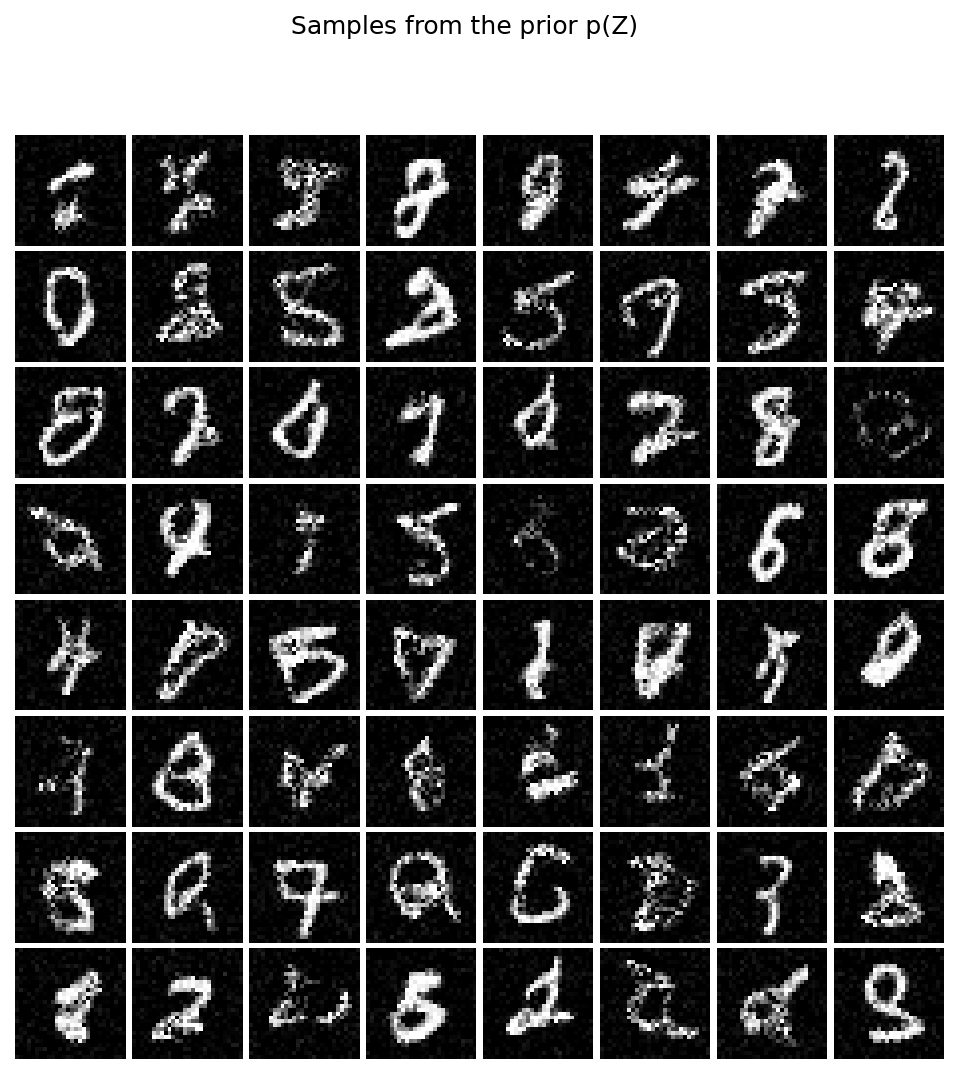
\includegraphics[width=0.6\textwidth]{outputs/task1_prior_samples.png}
    \caption{Images generated by sampling $\bz$ from the prior $p(\bZ)$,
    decoding, and sampling $\bx' \sim p(\bX \mid \bz)$.}
    \label{fig:prior}
\end{figure}

%% ===========================================================================
\section{Task 2 --- Choice of Conditional Data Distributions}
%% ===========================================================================

\section*{Task 2a --- Reflection on the Gaussian choice}
\addcontentsline{toc}{section}{Task 2a --- Reflection on the Gaussian choice}

The Gaussian likelihood is \emph{not fully appropriate} for MNIST for two reasons.
First, the Gaussian distribution is supported on all of $\mathbb{R}$, whereas pixel
values are bounded to $[0, 1]$; the decoder must therefore impose an \emph{ad hoc}
constraint (sigmoid on the mean, clamping of the predicted variance) that is not
required by the model itself.  Second, MNIST pixels are highly bimodal: they are
concentrated near $0$ (background) and $1$ (foreground), not spread over $[0, 1]$
like a Gaussian would predict.  Distributions that are either natively bounded (Beta)
or discrete (Bernoulli, Categorical) are a better fit for this data.

\section*{Task 2b --- Beta Distributions}
\addcontentsline{toc}{section}{Task 2b --- Beta Distributions}

\paragraph{Conditional log-likelihood.}
We replace the Gaussian conditional with a product of independent Beta distributions,
\[
p(\bX \mid \bz)
= \prod_{d=1}^{D} \mathrm{Beta}\!\big(X_d \mid \alpha_d(\bz),\, \beta_d(\bz)\big),
\]
where $\alpha_d(\bz)>0$ and $\beta_d(\bz)>0$ are the outputs of the decoder.
The log-likelihood of a single data-point $\bx$ given $\bz$ is
\begin{align}
\log p(\bx \mid \bz)
&= \sum_{d=1}^{D} \log \mathrm{Beta}\!\big(x_d \mid \alpha_d(\bz), \beta_d(\bz)\big) \nonumber \\
&= \sum_{d=1}^{D} \Big[
    (\alpha_d(\bz)-1)\log x_d
    + (\beta_d(\bz)-1)\log(1-x_d)
    - \log B\!\big(\alpha_d(\bz), \beta_d(\bz)\big)
   \Big],
\end{align}
where $\log B(\alpha,\beta) = \log\Gamma(\alpha) + \log\Gamma(\beta) - \log\Gamma(\alpha+\beta)$
is evaluated with \texttt{torch.lgamma} for numerical stability.  Because the Beta
distribution is only defined for $x_d \in (0, 1)$, we clamp pixel values to
$(\varepsilon, 1-\varepsilon)$ with $\varepsilon = 10^{-6}$ before computing
the log.

\paragraph{Decoder changes.}
The upsample path is identical to Task~1. The two output heads (\texttt{head\_mean},
\texttt{head\_logvar}) are replaced by \texttt{head\_alpha} and \texttt{head\_beta},
each followed by a \texttt{softplus} activation plus a small floor $10^{-6}$ to
guarantee strict positivity:

\begin{lstlisting}[caption={Beta decoder output heads (\texttt{vae/model\_beta.py}).}]
self.head_alpha = nn.Conv2d(32, 1, kernel_size=1)
self.head_beta  = nn.Conv2d(32, 1, kernel_size=1)

def forward(self, z):
    h = self.upsample(self.project(z).view(-1, 128, 4, 4))
    alpha = F.softplus(self.head_alpha(h)) + 1e-6   # alpha > 0
    beta  = F.softplus(self.head_beta(h))  + 1e-6   # beta  > 0
    return BetaParams(alpha=alpha, beta=beta)
\end{lstlisting}

\begin{lstlisting}[caption={Beta log-likelihood (\texttt{vae/elbo.py}).}]
def beta_log_likelihood(x, px, eps=1e-6):
    x_safe = x.clamp(eps, 1.0 - eps)
    log_prob = ((px.alpha - 1.0) * torch.log(x_safe)
                + (px.beta - 1.0) * torch.log(1.0 - x_safe))
    log_beta_fn = (torch.lgamma(px.alpha) + torch.lgamma(px.beta)
                   - torch.lgamma(px.alpha + px.beta))
    return (log_prob - log_beta_fn).flatten(start_dim=1).sum(dim=1)
\end{lstlisting}

The encoder is unchanged.  For visualisation we use the posterior mean
$\mathbb{E}[\mathrm{Beta}(\alpha,\beta)] = \alpha/(\alpha+\beta)$, which gives
sharper images than sampling from the Beta distribution.

\paragraph{Training.}
We used the same hyperparameters as Task~1 (Adam, $\text{lr}=10^{-3}$, batch 128,
patience 5). Training stopped at epoch~51 (best validation ELBO $\mathbf{7585.3}$
at epoch~46). Note that the Beta ELBO is on a different scale than the Gaussian ELBO
from Task~1 because the Beta log-likelihood also contains the normalisation term
$-\log B(\alpha,\beta)$.

\begin{figure}[h]
    \centering
    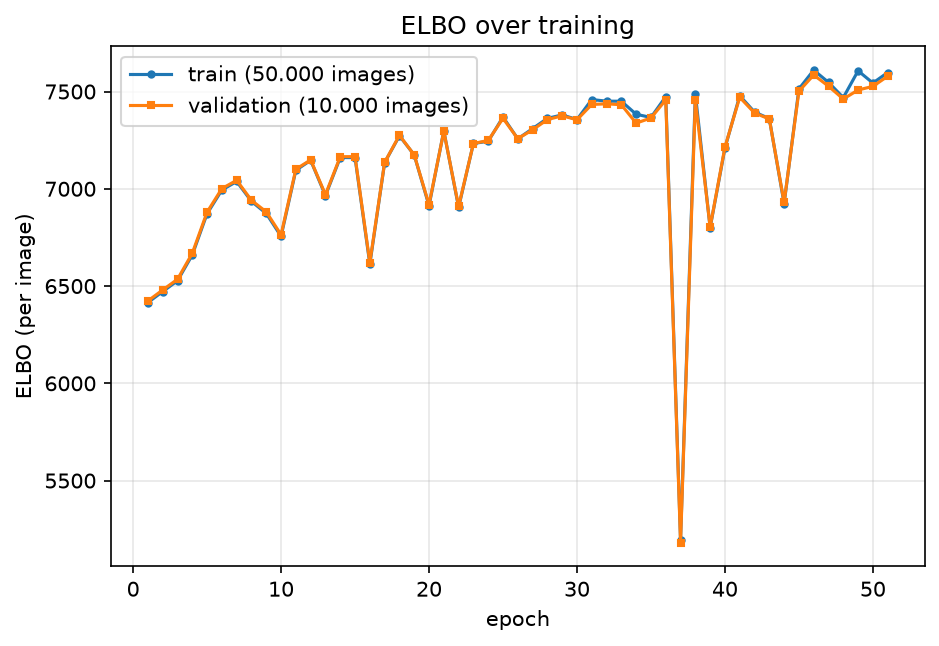
\includegraphics[width=0.75\textwidth]{outputs/task2b_elbo.png}
    \caption{Task 2b -- ELBO (per image) for the Beta VAE on the training and
    validation splits as a function of the training epoch.}
    \label{fig:beta_elbo}
\end{figure}

\begin{figure}[h]
    \centering
    \begin{subfigure}[b]{0.48\textwidth}
        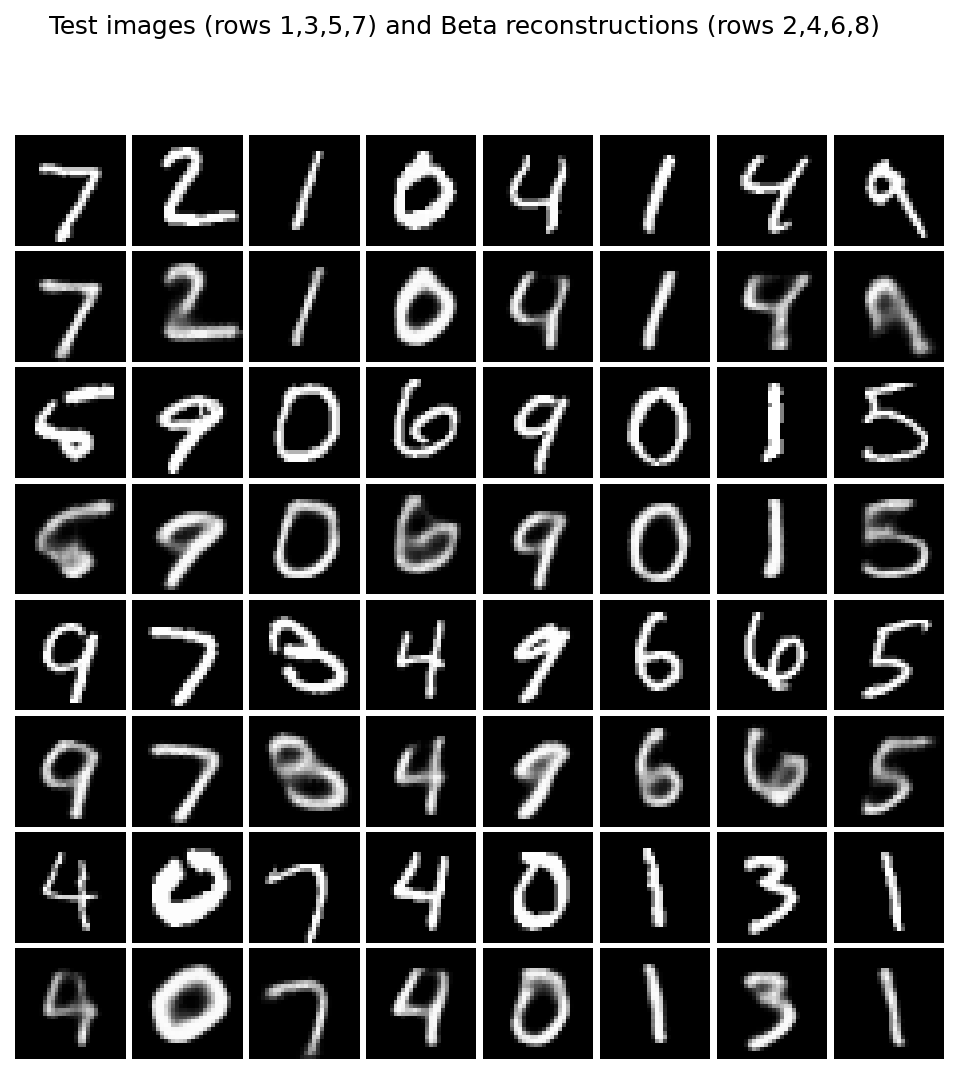
\includegraphics[width=\textwidth]{outputs/task2b_reconstructions.png}
        \caption{Reconstructions (posterior mean $\alpha/(\alpha+\beta)$).}
    \end{subfigure}
    \hfill
    \begin{subfigure}[b]{0.48\textwidth}
        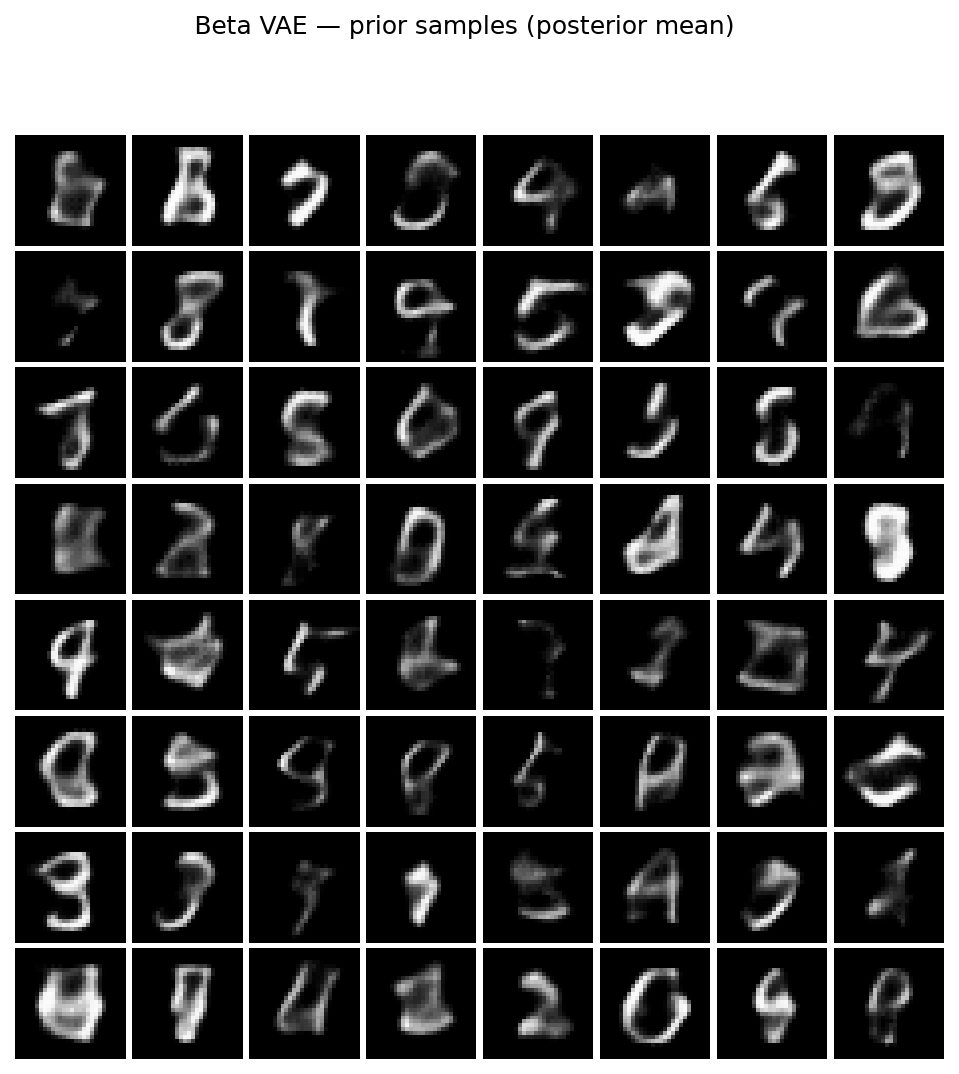
\includegraphics[width=\textwidth]{outputs/task2b_prior_samples.png}
        \caption{Prior samples.}
    \end{subfigure}
    \caption{Task 2b -- Beta VAE: test-image reconstructions (left) and images
    sampled from $p(\bZ)$ (right). In both cases we display the posterior mean
    $\alpha_d(\bz)/(\alpha_d(\bz)+\beta_d(\bz))$ rather than a stochastic sample.}
    \label{fig:beta_recon}
\end{figure}

\section*{Task 2c --- Categorical Distributions}
\addcontentsline{toc}{section}{Task 2c --- Categorical Distributions}

\paragraph{Discretisation.}
We discretise each pixel into $k=4$ equal-width bins:
\begin{center}
\begin{tabular}{lll}
\hline
Bin & Range & Midpoint \\
\hline
0 & $[0.00, 0.25)$ & $0.125$ \\
1 & $[0.25, 0.50)$ & $0.375$ \\
2 & $[0.50, 0.75)$ & $0.625$ \\
3 & $[0.75, 1.00]$ & $0.875$ \\
\hline
\end{tabular}
\end{center}
We chose $k=4$ because MNIST pixels are bimodal (mostly near 0 or 1): four bins
capture this bimodality while keeping the output head compact.  Using more bins
(e.g.\ 256) would require a much larger output head and offer diminishing returns,
since intermediate gray values are rare.

\paragraph{Conditional log-likelihood.}
Let $\mathrm{bin}(x_d) \in \{0,\ldots,k-1\}$ be the bin index of pixel $x_d$.
The conditional log-likelihood is
\[
\log p(\bx \mid \bz)
= \sum_{d=1}^{D} \log \mathrm{Cat}\!\big(\mathrm{bin}(x_d) \mid \bm{\pi}_d(\bz)\big)
= \sum_{d=1}^{D} \log \pi_{d,\,\mathrm{bin}(x_d)}(\bz),
\]
where $\bm{\pi}_d(\bz) = \mathrm{softmax}(\mathrm{logits}_d(\bz)) \in \Delta^{k-1}$
is the categorical probability vector for pixel $d$.

\paragraph{Decoder changes.}
The upsample path is identical to Task~1. The two 1-channel heads are replaced by a
single $k$-channel head whose outputs are raw logits:

\begin{lstlisting}[caption={Categorical decoder (\texttt{vae/model\_categorical.py}).}]
self.head_logits = nn.Conv2d(32, k, kernel_size=1)  # k=4 channels

def forward(self, z):
    h = self.upsample(self.project(z).view(-1, 128, 4, 4))
    return self.head_logits(h)   # raw logits, shape (B, k, H, W)
\end{lstlisting}

\begin{lstlisting}[caption={Categorical log-likelihood (\texttt{vae/elbo.py}).}]
def cat_log_likelihood(x, logits, k):
    x_bins = (x * k).long().clamp(0, k - 1).squeeze(1)  # (B, H, W)
    log_probs = F.log_softmax(logits, dim=1)             # (B, k, H, W)
    nll = F.nll_loss(log_probs, x_bins, reduction="none")
    return -nll.flatten(start_dim=1).sum(dim=1)
\end{lstlisting}

For reconstruction and sampling we translate bin probabilities back to pixel
values using the \emph{expected value}: $\hat{x}_d = \sum_{i=0}^{k-1} \pi_{d,i} \cdot m_i$,
where $m_i = (i + 0.5)/k$ is the midpoint of bin $i$.

\paragraph{Training.}
Training stopped at epoch~44 (best validation ELBO $\mathbf{-146.1}$ at epoch~39).
The ELBO values are negative and of a different order of magnitude than
the other models because the log-likelihood is computed over discrete bins rather
than continuous densities.

\begin{figure}[h]
    \centering
    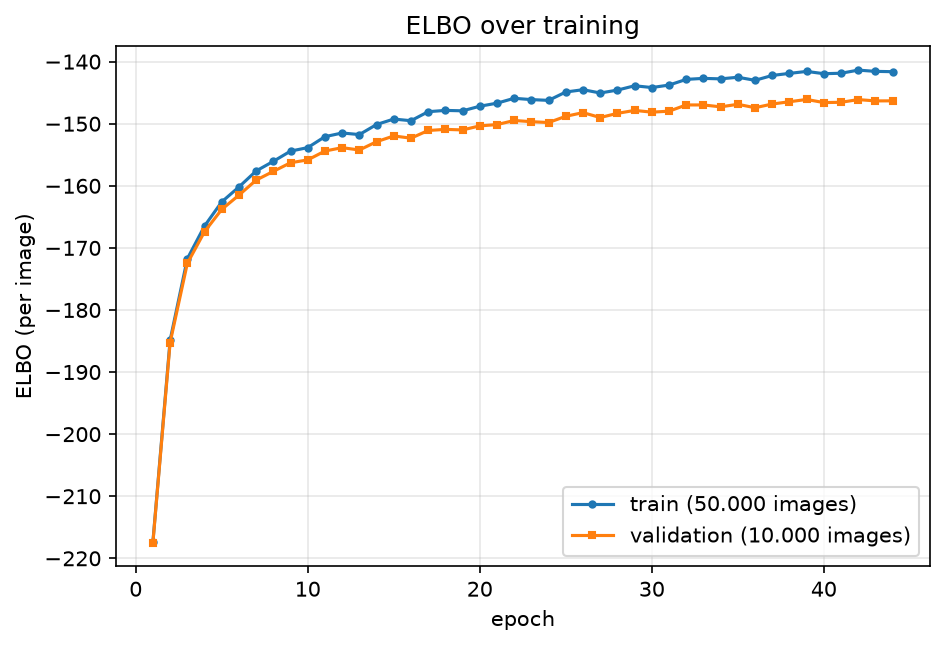
\includegraphics[width=0.75\textwidth]{outputs/task2c_elbo.png}
    \caption{Task 2c -- ELBO (per image) for the Categorical VAE on the training and
    validation splits as a function of the training epoch.}
    \label{fig:cat_elbo}
\end{figure}

\begin{figure}[h]
    \centering
    \begin{subfigure}[b]{0.48\textwidth}
        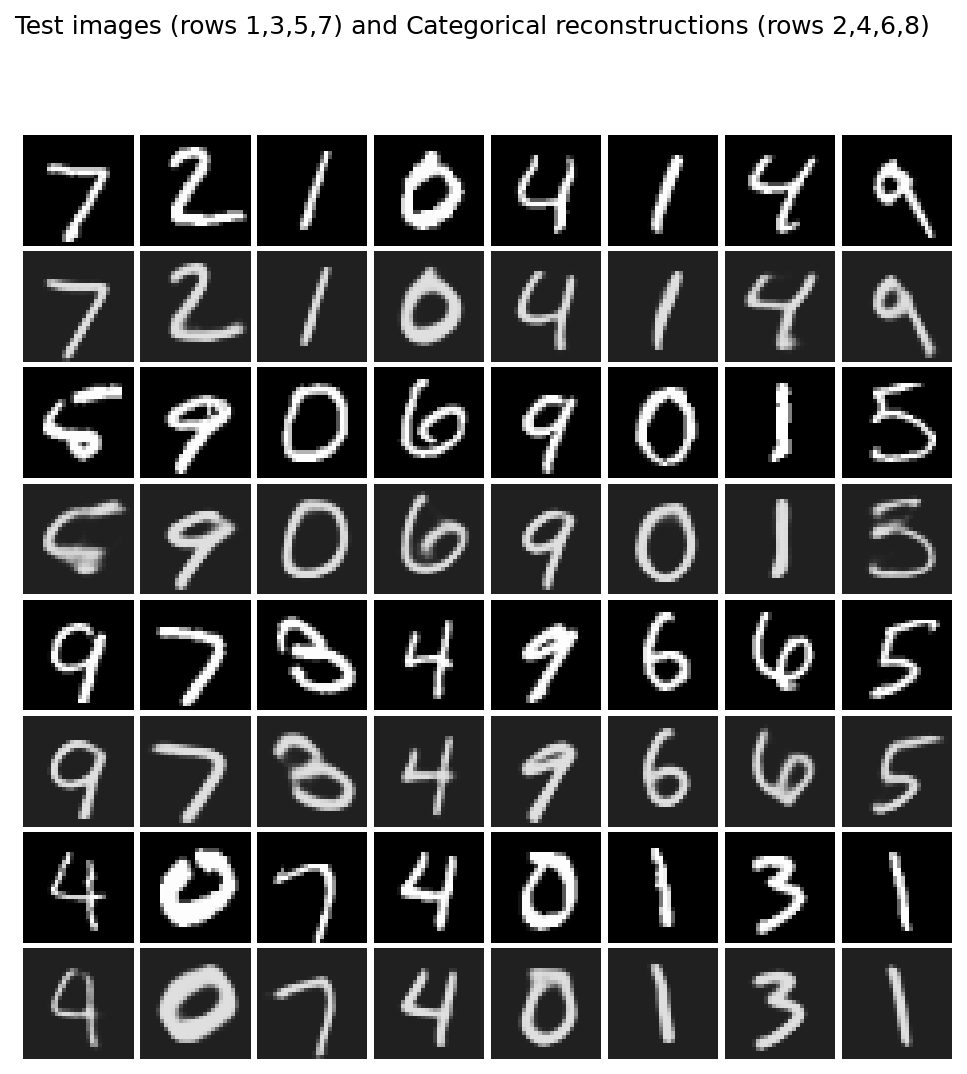
\includegraphics[width=\textwidth]{outputs/task2c_reconstructions.png}
        \caption{Reconstructions (expected pixel value).}
    \end{subfigure}
    \hfill
    \begin{subfigure}[b]{0.48\textwidth}
        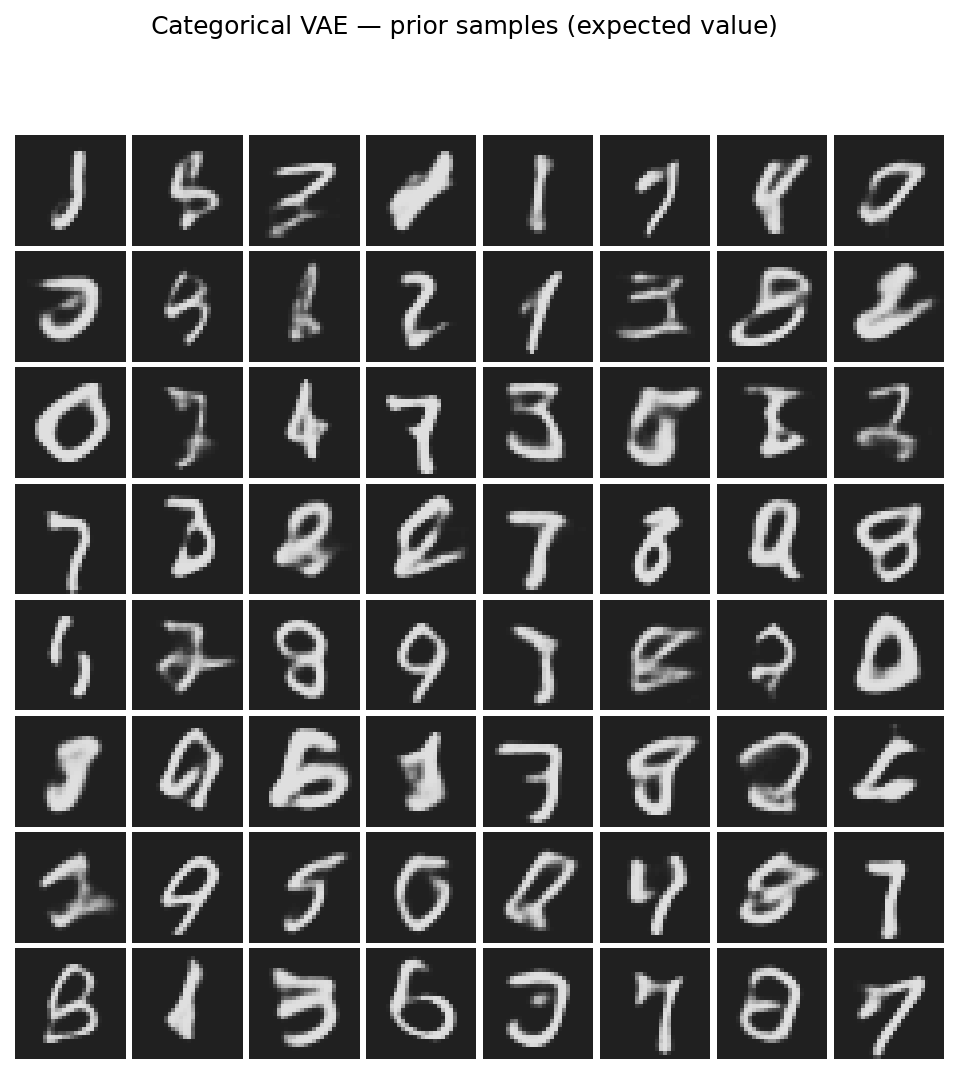
\includegraphics[width=\textwidth]{outputs/task2c_prior_samples.png}
        \caption{Prior samples.}
    \end{subfigure}
    \caption{Task 2c -- Categorical VAE: test-image reconstructions (left) and images
    sampled from $p(\bZ)$ (right). Pixel values are computed as the weighted sum of
    bin midpoints under the predicted categorical distribution.}
    \label{fig:cat_recon}
\end{figure}

\section*{Task 2d --- Bernoulli Distributions}
\addcontentsline{toc}{section}{Task 2d --- Bernoulli Distributions}

\paragraph{Model and objective.}
The decoder now produces a Bernoulli probability $\pi_d(\bz) \in (0,1)$ per pixel.
Training maximises
\[
-H\!\big(p(\bB \mid \bx),\, p(\bB \mid \bz)\big) - \KL\!\big(q(\bZ \mid \bx)\,\|\,p(\bZ)\big),
\]
where the \emph{negative cross-entropy} between the two Bernoulli distributions
$p(\bB \mid \bx) = \prod_d \mathrm{Bern}(B_d \mid x_d)$ and
$p(\bB \mid \bz) = \prod_d \mathrm{Bern}(B_d \mid \pi_d(\bz))$ is
\begin{equation}
-H\!\big(p(\bB \mid \bx),\, p(\bB \mid \bz)\big)
= \sum_{d=1}^{D} \Big[ x_d \log \pi_d(\bz) + (1 - x_d) \log\!\big(1 - \pi_d(\bz)\big) \Big].
\end{equation}
This is exactly the negative binary cross-entropy (BCE), implemented with
\texttt{binary\_cross\_entropy\_with\_logits} for numerical stability.

\paragraph{Decoder changes.}
The decoder produces a single raw logit per pixel (no activation); the sigmoid
$\pi_d = \sigma(\mathrm{logit}_d)$ is applied inside the loss function.

\begin{lstlisting}[caption={Bernoulli decoder (\texttt{vae/model\_bernoulli.py}).}]
self.head_logits = nn.Conv2d(32, 1, kernel_size=1)  # raw logit per pixel

def forward(self, z):
    h = self.upsample(self.project(z).view(-1, 128, 4, 4))
    return self.head_logits(h)   # shape (B, 1, H, W)
\end{lstlisting}

\begin{lstlisting}[caption={Bernoulli (cross-entropy) objective (\texttt{vae/elbo.py}).}]
def bernoulli_neg_cross_entropy(x, logits):
    neg_ce = -F.binary_cross_entropy_with_logits(
        logits, x, reduction="none")
    return neg_ce.flatten(start_dim=1).sum(dim=1)
\end{lstlisting}

For reconstruction and sampling we use the posterior mean
$\mathbb{E}[B_d \mid \bz] = \pi_d(\bz) = \sigma(\mathrm{logit}_d(\bz))$ rather than
sampling, which produces sharper, less noisy images (as suggested in the hint).

\paragraph{Training.}
Training stopped at epoch~68 (best validation objective $\mathbf{-95.1}$ at
epoch~63). The objective is measured in nats and reflects the cross-entropy between
the data distribution and the model, not a conventional log-likelihood density.

\begin{figure}[h]
    \centering
    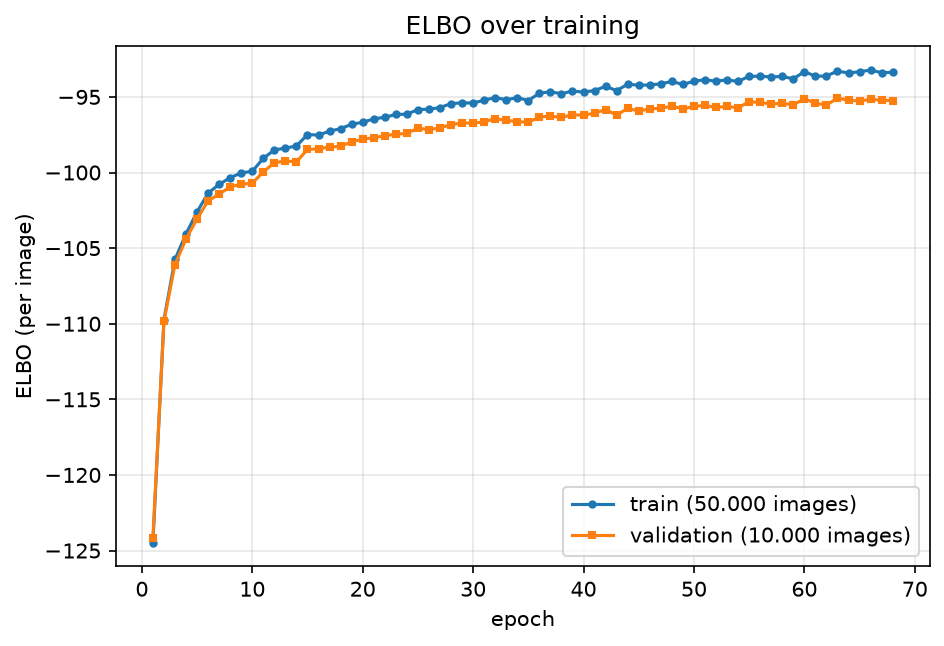
\includegraphics[width=0.75\textwidth]{outputs/task2d_elbo.png}
    \caption{Task 2d -- Modified ELBO (per image) for the Bernoulli VAE on the
    training and validation splits as a function of the training epoch.}
    \label{fig:bern_elbo}
\end{figure}

\begin{figure}[h]
    \centering
    \begin{subfigure}[b]{0.48\textwidth}
        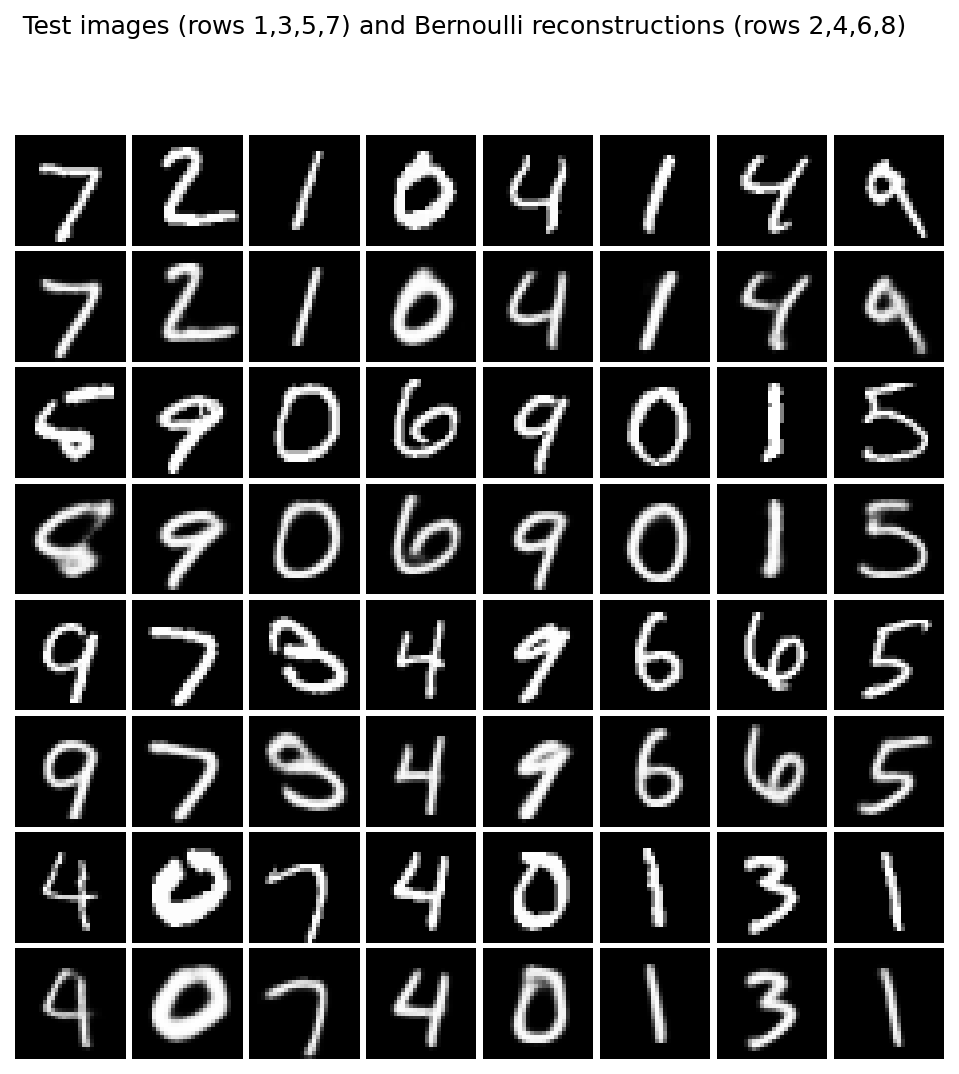
\includegraphics[width=\textwidth]{outputs/task2d_reconstructions.png}
        \caption{Reconstructions (posterior mean $\pi_d(\bz)$).}
    \end{subfigure}
    \hfill
    \begin{subfigure}[b]{0.48\textwidth}
        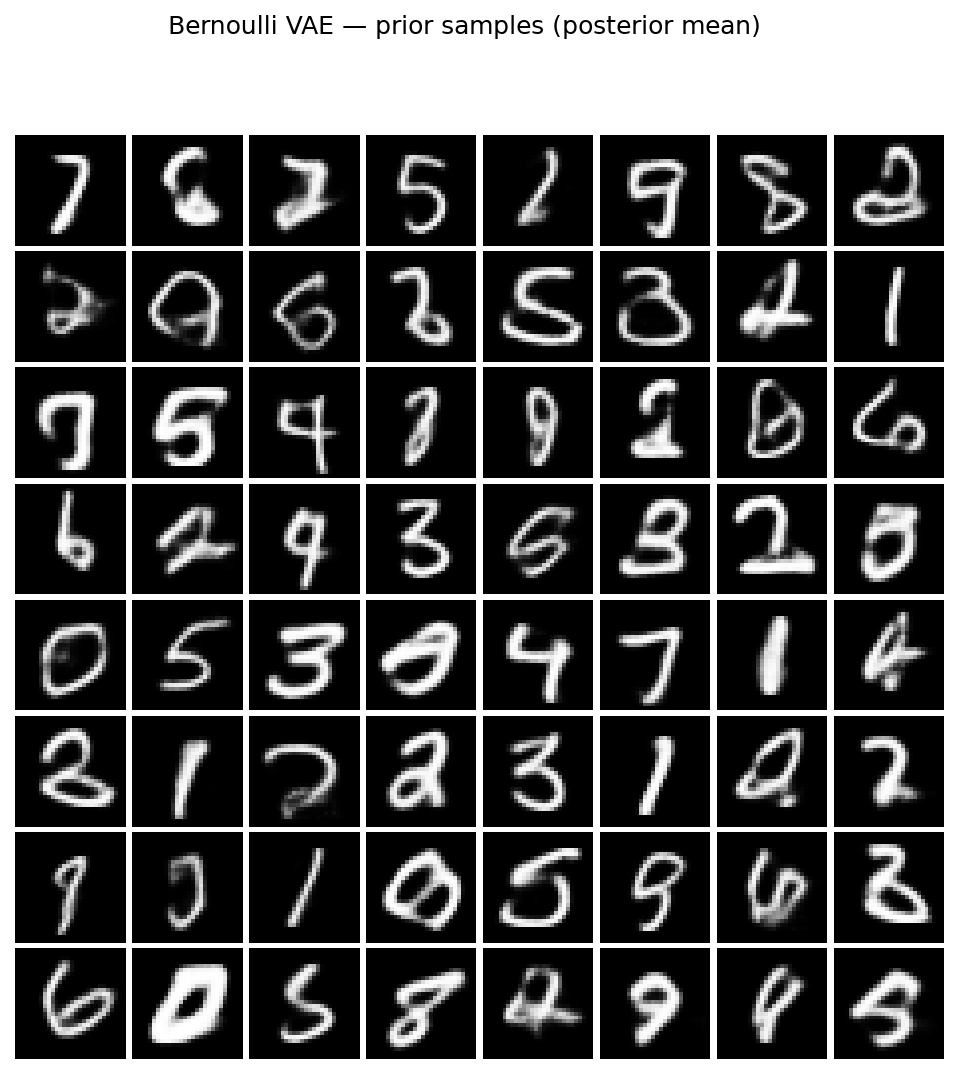
\includegraphics[width=\textwidth]{outputs/task2d_prior_samples.png}
        \caption{Prior samples.}
    \end{subfigure}
    \caption{Task 2d -- Bernoulli VAE: test-image reconstructions (left) and images
    sampled from $p(\bZ)$ (right). We display $\pi_d(\bz) = \sigma(\mathrm{logit}_d(\bz))$
    (the posterior mean) rather than binary samples.}
    \label{fig:bern_recon}
\end{figure}

\section*{Task 2e --- Reflection on the best choice of distribution}
\addcontentsline{toc}{section}{Task 2e --- Reflection on the best choice of distribution}

Among the four distributions considered, we argue that the \textbf{Bernoulli} model
provides the most \emph{practically} appropriate choice for MNIST, while the
\textbf{Beta} is most \emph{theoretically} motivated.

\paragraph{Bernoulli.}
MNIST digits are nearly binary: the vast majority of pixels are either
close to 0 (background) or close to 1 (foreground), with few intermediate values.
The Bernoulli model matches this prior knowledge perfectly, and its cross-entropy
objective is equivalent to maximising the probability of the correct binary
``on/off'' interpretation of each pixel.  The resulting reconstructions
(Figure~\ref{fig:bern_recon}) are visually crisp and faithful.

\paragraph{Beta.}
From a theoretical standpoint the Beta distribution is the natural choice: it
is supported on $(0,1)$, its two shape parameters give it great flexibility
(it can represent unimodal, bimodal and uniform shapes), and it explicitly
treats pixel values as continuous probabilities in $[0,1]$.  In practice,
however, the presence of the log-Beta normalisation term and the need to clamp
pixel values away from the boundary add numerical complexity.

\paragraph{Categorical.}
The Categorical model is a flexible, parameter-free approximation to any
distribution over $[0,1]$; it is not constrained to any particular shape.
Its main disadvantage is that the choice of $k$ and the bin boundaries are
hyper-parameters, and the discrete representation discards metric structure
between adjacent bins.

\paragraph{Gaussian.}
Although computationally simple, the Gaussian likelihood is the least
appropriate: its unbounded support is a structural mismatch with pixel
data in $[0,1]$, and the model must resort to architectural constraints
(sigmoid on the mean, clamped log-variance) that are not demanded by the data.

\paragraph{Alternative: Logistic or Continuous Bernoulli.}
A distribution not covered above that is arguably \emph{more} appropriate is the
\textbf{Continuous Bernoulli} (Loaiza-Ganem \& Cunningham, 2019), which is defined
exactly on $[0,1]$, has a single natural parameter $\lambda$, and is closely related
to the Bernoulli model used here.  Unlike the standard Bernoulli cross-entropy
objective, the Continuous Bernoulli adds a normalisation term that accounts for the
fact that the data are continuous, leading to a proper probability density on $[0,1]$.

\end{document}
